\documentclass[12pt]{article}
\usepackage{times} 			% use Times New Roman font

\usepackage[margin=1in]{geometry}   % sets 1 inch margins on all sides
\usepackage{hyperref}               % for URL formatting
\usepackage[pdftex]{graphicx}       % So includegraphics will work
\setlength{\parskip}{1em}           % skip 1em between paragraphs
\usepackage{indentfirst}            % indent the first line of each paragraph
\usepackage{datetime}
\usepackage[small, bf]{caption}
\usepackage{listings}               % for code listings
\usepackage{xcolor}                 % for styling code
\usepackage{multirow}
\usepackage{float}
\usepackage{csvsimple}
\usepackage{ragged2e}
\usepackage{cite}

%New colors defined below
\definecolor{backcolour}{RGB}{246, 246, 246}   % 0xF6, 0xF6, 0xF6
\definecolor{codegreen}{RGB}{16, 124, 2}       % 0x10, 0x7C, 0x02
\definecolor{codepurple}{RGB}{170, 0, 217}     % 0xAA, 0x00, 0xD9
\definecolor{codered}{RGB}{154, 0, 18}         % 0x9A, 0x00, 0x12

%Code listing style named "gcolabstyle" - matches Google Colab
\lstdefinestyle{gcolabstyle}{
  basicstyle=\ttfamily\small,
  backgroundcolor=\color{backcolour},   
  commentstyle=\itshape\color{codegreen},
  keywordstyle=\color{codepurple},
  stringstyle=\color{codered},
  numberstyle=\ttfamily\footnotesize\color{darkgray}, 
  breakatwhitespace=false,         
  breaklines=true,                 
  captionpos=b,                    
  keepspaces=true,                 
  numbers=left,                    
  numbersep=5pt,                  
  showspaces=false,                
  showstringspaces=false,
  showtabs=false,                  
  tabsize=2
}

\lstset{style=gcolabstyle}      %set gcolabstyle code listing

% for fancy page headings
\usepackage{fancyhdr}
\setlength{\headheight}{13.6pt} % to remove fancyhdr warning
\pagestyle{fancy}
\fancyhf{}
\rhead{\small \thepage}
\lhead{\small Documentation}  % EDIT THIS
\chead{\small JetPack Compose and RoomDatabase Design Practices} 

%-------------------------------------------------------------------------
\begin{document}

\begin{centering}
{\large\textbf{Android Template Code}}\\ % EDIT THIS
                                % REPLACE # with HW num and ADD title
Jacob Conner\\                     % EDIT THIS
October 7, 2021\\                      % EDIT THIS
\end{centering}

%-------------------------------------------------------------------------
\tableofcontents

% The * after \section just says to not number the sections
\section{Gradle}
This section examines the \textit{build.gradle} files in the Project and App folders and the project \textit{Build.settings} files. 
\newpage
\subsection{ProjectBuildGradle}
\lstinputlisting[language=Java, caption=Project build.gradle file, label={lst:projectBuildGradle}]{build.gradle}
All Android projects consist of at least two \textit{build.gradle} files, a project level \textit{build.gradle} file and an application level \textit{build.gradle} file. The project level \textit{build.gradle} file is shown in Listing  \ref{lst:projectBuildGradle}. Generally this 
\textit{build.gradle} file contains a \verb|buildscript| tag that has a number of subsections. The section mostly likely to be 
editted is the \verb|ext| section. In this section gradle environment variables can be defined particularly to keep track 
of versions of various dependencies. In this example the \verb|compose_version| variable is defined with \verb|compose_version = '1.0.1'|. Dependencies can be defined in this section but generally should be defined using the application level \textit{build.gradle} file. 

\newpage

\subsection{AppBuildGradle}
\lstinputlisting[language=Java, caption=App build.gradle file, label={lst:appBuildGradle}]{app/build.gradle}
This app-level  \textit{build.gradle} file is used to define the various plugins, application dependencies and gradle scripts pertinent to the application. In the example file in Listing \ref{lst:appBuildGradle} the file starts with plugins section. The plugins section consists of four plugins.:
\begin{itemize}
    \item com.android.application
    \item kotlin-android
    \item Kapt plugin - kotlin-kapt
    \item Dokka plugin - org.jetbrains.dokka
\end{itemize}
\verb|com.android.application| and \verb|kotlin-android| are all included in the application by default. This example has added the plugin \verb|kotlin-kapt| to enable the program to load the room compiler dependency using the kapt command. The dokka plugin needed to create documentation using KDoc is added with the \verb|id("org.jetbrains.dokka") version "1.4.0"|.
Various gradle tasks should be added in the application \textit{build.gradle} file. 
\begin{lstlisting}[numbers=none, 
			caption=Task to generate Dokka documentation,
			label={lst:dokkatask}]
tasks.dokkaHtml.configure {
    outputDirectory.set(file("../documentation/html"))
}
\end{lstlisting}
The task to generate dokka documentation is defined using the code in Listing \ref{lst:dokkatask} . Gradle documentation can be created using the terminal with the command \verb|gradlew dokkaHtml|. Dokka will then parse all KDoc comment lines in Kotlin classes and generate the documentation in the build/dokka folder. 

Dependencies are stored in the dependencies section of the \textit{build.gradle} file. When a new empty compose application is created, a number of compose dependencies are included as well as various testing frameworks. The Jetpack compose navigation library and the jetpack compose lifecycle libraries are not included by default but are present in the example app \textit{build.gradle} file. The project also makes use of RoomDatabase library so those libraries are included. In order to allow for the downloading and display of images from the internet the \verb|io.coil-kt:coil-compose| library is included. 


\newpage
\section{AndroidManifest}
\lstinputlisting[language=xml, caption=Android Manifests File, label={lst:androidXML}]{app/src/main/AndroidManifest.xml}
The \textit{android.manifest} file shown in \ref{lst:androidXML} provides information about the various permissions in the application. 

\begin{lstlisting}[numbers=none, 
			caption=Line to give permission to allow internet access,
			label={lst:internetPermission}]
<uses-permission android:name="android.permission.INTERNET" />
\end{lstlisting}

\begin{lstlisting}[numbers=none, 
			caption=Line to give permission to allow network access,
			label={lst:networkPermission}]
<uses-permission android:name="android.permission.ACCESS_NETWORK_STATE"/>
\end{lstlisting}
The most common reason to edit this file is when an application needs to have access to a website or other resource. Internet access is enabled with the line shown in Listing \ref{lst:internetPermission}.
Network access is also needed to allow the application to access the web, and this is enabled with the line in Listing \ref{lst:networkPermission}.


\newpage

\section{RoomDatabase}
The RoomDatabase library is an object relational mapping (ORM) library in Android that serves as a layer for SQLite queries \cite{GoogleRoomDB} .
\subsection{Dependencies}
The implementations are briefly discussed in Section \ref{lst:appBuildGradle}, but a list of the required implementations in the \textit{build.gradle} file are listed below. 

\begin{itemize}
\item RoomDatabase Libraries \begin{itemize}
    \item implementation "androidx.room:room-runtime:\$room\_version"
    \item annotationProcessor "androidx.room:room-compiler:\$room\_version"
    \item implementation "androidx.room:room-ktx:2.3.0"
    \item kapt "androidx.room:room-compiler:2.3.0"
    \end{itemize}
 \item Lifecycle Libraries \begin{itemize}
    \item implementation "androidx.compose.runtime:runtime-livedata:\$compose\_version"
    \item implementation "androidx.lifecycle:lifecycle-livedata-ktx:2.3.1"
    \end{itemize}
\end{itemize}
 \newpage
 
 The model view view model approach taken in this document is largely derived from the Make it Easy tutorial \cite{MakeItEasyRoom1} \cite{MakeItEasyRoom2} \cite{RoomCodeLab}.
 \subsection{Entities}
The lowest level of RoomDatabase is the entity or data model. An entity is simply a data class that describes the schema for a time using Room annotations. The contents of each entity should correspond to the columns of a single SQLite table. 
\lstinputlisting[language=Java, caption=Example entity class, label={lst:exampleEntity}]{app/src/main/java/com/example/roomandapi/entity/TeamMember.kt}

In Listing \ref{lst:exampleEntity}, an example entity class \verb|TeamMember| is provided for a table called team that stores information about members of a team. In this class, the first Room notation encountered is the \verb|@Entity|notation. This notation is called before the data class is defined and is used to help the Room library identify where this model's data will reside in the SQLite database. In this case the table is called \verb|Team| but the data class is called \verb|TeamMember|. 
Next the data class is created using the \verb|data class <nameOfClass>( <contents>)|. It is important to note that a data class in Kotlin does not contain any methods and is simply defined with the parameters using the parentheses that initialize it. 

The next annotation used in this example class is \verb|@PrimaryKey|. This annotation is used to define the column below as a primary key for the table, which means it has to be unique and cannot be null. The notation also has the possible parameter of \verb|(autoGenerate = true)| which advises SQLite to autoincrement that column. 
The last annotation in the example entity class is \verb|@ColumnInfo| which is used to define the name of the table column using the parameter \verb|name="<nameOfColumn>"|. Once the column name has been defined, a variable in kotlin is created for the model which is tied to the table column set. This process is repeated for all columns needed in the table and each column is separated by commas (","). 
 
\subsection{DAO}
Once an entity has been created, a data abstraction object (DAO) has to be created. This is an interface for the entity that maps SQL queries to various methods that can be called. 
\lstinputlisting[language=Java, caption=Example DAO, label={lst:exampleDAO}]{app/src/main/java/com/example/roomandapi/dao/TeamMemberDAO.kt}

An example of an DAO interface is shown in Listing \ref{lst:exampleDAO}. In this file, the interface is annotated as a DAO with the \verb|@DAO| annotation. After the interface header is created with \verb|interface <nameOfDAO>| the various SQL methods are defined with an annotation followed by a method. The first type of SQL Query annotation is \verb|@Query\verb. This annotation takes a SQL query as a parameter.  Then immediately below it, a function is defined that will handle that query and return either an entity or a list of some sort. The \verb|@Query\verb supports parameterized sql queries as shown in the \verb|getById function| and the parameter in the query is used as a parameter in the method tied to that query. 
Room provides a few SQL query annotations that do not require you to specifically type out the SQL query. The \verb|@Insert| annotation takes a list of entities and inserts them into a database using the method below. The option parameter \verb|onConflict = OnConflictStrategy.REPLACE| allows you to specify the conflict strategy with foreign key constraints when a value is inserted.  The \verb|@Update| annotation is used to create an update query where an entity is provided and the values of the entity are used to update the value of the entity in the database. The  annotation  \verb|@Delete|  writes the query to delete the entity in the database that matches the entity provided in the method. 

\subsection{Repository}
\lstinputlisting[language=Java, caption=Example repository class, label={lst:exampleRepo}]{app/src/main/java/com/example/roomandapi/repository/TeamMemberRepository.kt}
In order to simplify the ability to to call the functions in the DAO interface, a repository class is created.An example repository is shown in Listing \ref{lst:exampleRepo}  This repository class takes the DAO interface as an argument. Class methods for each of the DAO functions. In order to support asynchronous methods since a SQL query may not run instantaneously, each method is marked with suspend. Suspend is part of the coroutines library and is used to force a method to run asynchronously on a coroutine. "A coroutine is an instance of suspendable  computation" that is "not bound to any particular thread" that can be suspended and resumed on different threads \cite{kotlinCoroutines}. 

\subsection{Database}
\lstinputlisting[language=Java, caption=Example database class, label={lst:exampleDB}]{app/src/main/java/com/example/roomandapi/database/WCDatabase.kt}

Listing \ref{lst:exampleDB} shows the database class. There should be one database class for each database in the project, but generally one database should suffice for most applications. The database class starts with the \verb|@Database| annotation which abstracts the requirements for any SQLite database using the SQLite connector in a given language. This annotation requires a list of entity classes in the database, a database version, and exportSchema. The database is an abstract class extending the RoomDatabase using the line \verb|abstract class <nameOfDatabase>: RoomDatabase()|. An abstract constructor for each DAO is provided to allow the database to access the sql queries needed by the entity managed by the DAO. The database class has one method, \verb|getInstance| which takes the context of the application. and returns a returns a database object. A database instance is created with the Room.databaseBuilder method and it takes the context of the application provided, the database class and a string with the name of the database. The synchronized method chains fallbackToDestructiveMigration(), which is used for migrations, when they fail and rebuilds the database if the migration fails. The build method is the method that actually builds the database \cite{roomDBMethods}. 

\subsection{Supporting Dates}
\lstinputlisting[language=Java, caption=Converter Class for supporting Dates, label={lst:exampleConverter}]{app/src/main/java/com/example/roomandapi/utility/DateTimeConverter.kt}

SQLite supports 5 data types. 
\begin{itemize}
\item NULL 
\item INTEGER
\item REAL
\item TEXT
\item BLOB
\end{itemize}
A notable omission in the SQLite database is the absence of a Date type. Dates are supported in a variety of ways. They can be stored as an INTEGER as timestamp with the seconds since January 1st, 1970. Another alternative is it can be stored as TEXT variable using ISO8601 strings such as "YYYY-MM-DD". A final option is the Date can be stored as Julian days numbers since November 24th 4714 BC. RoomDatabase does not provide out of the box support for dates likely due to the variety of options to store Dates in SQLite \cite{SqliteDataTypes}. Instead the developer has to create a helper converter class to convert the type of Date variable used in Kotlin to the type used in the SQLite design \cite{RoomDBTypeConverters} \cite{LuaSoftwareLocalDateTime}. 

In Listing \ref{lst:exampleConverter} an example type converter is provided to convert a date string formatted using the ISO86601 LOCAL\_DATE string. This class contains a formatter which is used to define how the DateTime string is formatted. There are numerous options for date time string formatting supported in Java and Kotlin \cite{DateTimeFormatterDocs} \cite{AndroidDateTimeFormatterDocs}. Once the formatting string has been defined, the converter class contains two methods for converting to and from the LocalDate class \cite{StackOverflowLocalDate}. 

\begin{lstlisting}[numbers=none, 
			caption=Task to generate Dokka documentation,
			label={lst:converterAnnotation}]
@TypeConverters(DateTimeConverter::class)
\end{lstlisting}

Once the converter class has been created, it needs to be added to the Database class shown in \ref{lst:exampleDB}.The \verb|@TypeConverters| annotation is used to allow the Database to support those conversions between SQLite types and Kotlin classes. This annotation is added before the database class header and takes the class for the file used as shown in Listing \ref{lst:converterAnnotation} 

\subsection{ViewModel}
\lstinputlisting[language=Java, caption=Example ViewModel class, label={lst:exampleViewModel}]{app/src/main/java/com/example/roomandapi/viewmodel/TeamMemberViewModel.kt}
The view model is the class that GUI will interact with to run queries. This final layer of abstraction 
The view model, class extends the AndroidViewModel class and takes the argument of application as the context. The init function initializes a DAO with the database class's get instance method using application as context and calls the teamMemberDao function to generate the Dao. 

\section{Testing Room}
In Android projects there are two types of unit tests. There are standard Unit Tests that make use of the JUnit library and run like a normal Java or Kotlin project would. The second type of test is the Android  Test which runs a virtualized environment to access the Android Libraries to run the functions that require the Android Framework to run \cite{AndroidTestingFundamentals}. Room Database is one of those examples. 

\subsection{Creating Tests}

\begin{figure}[H]
    \centering
    % trim and clip are used to crop the image, trim=left bottom right top
    % width sets max width, height will be scaled appropriately
    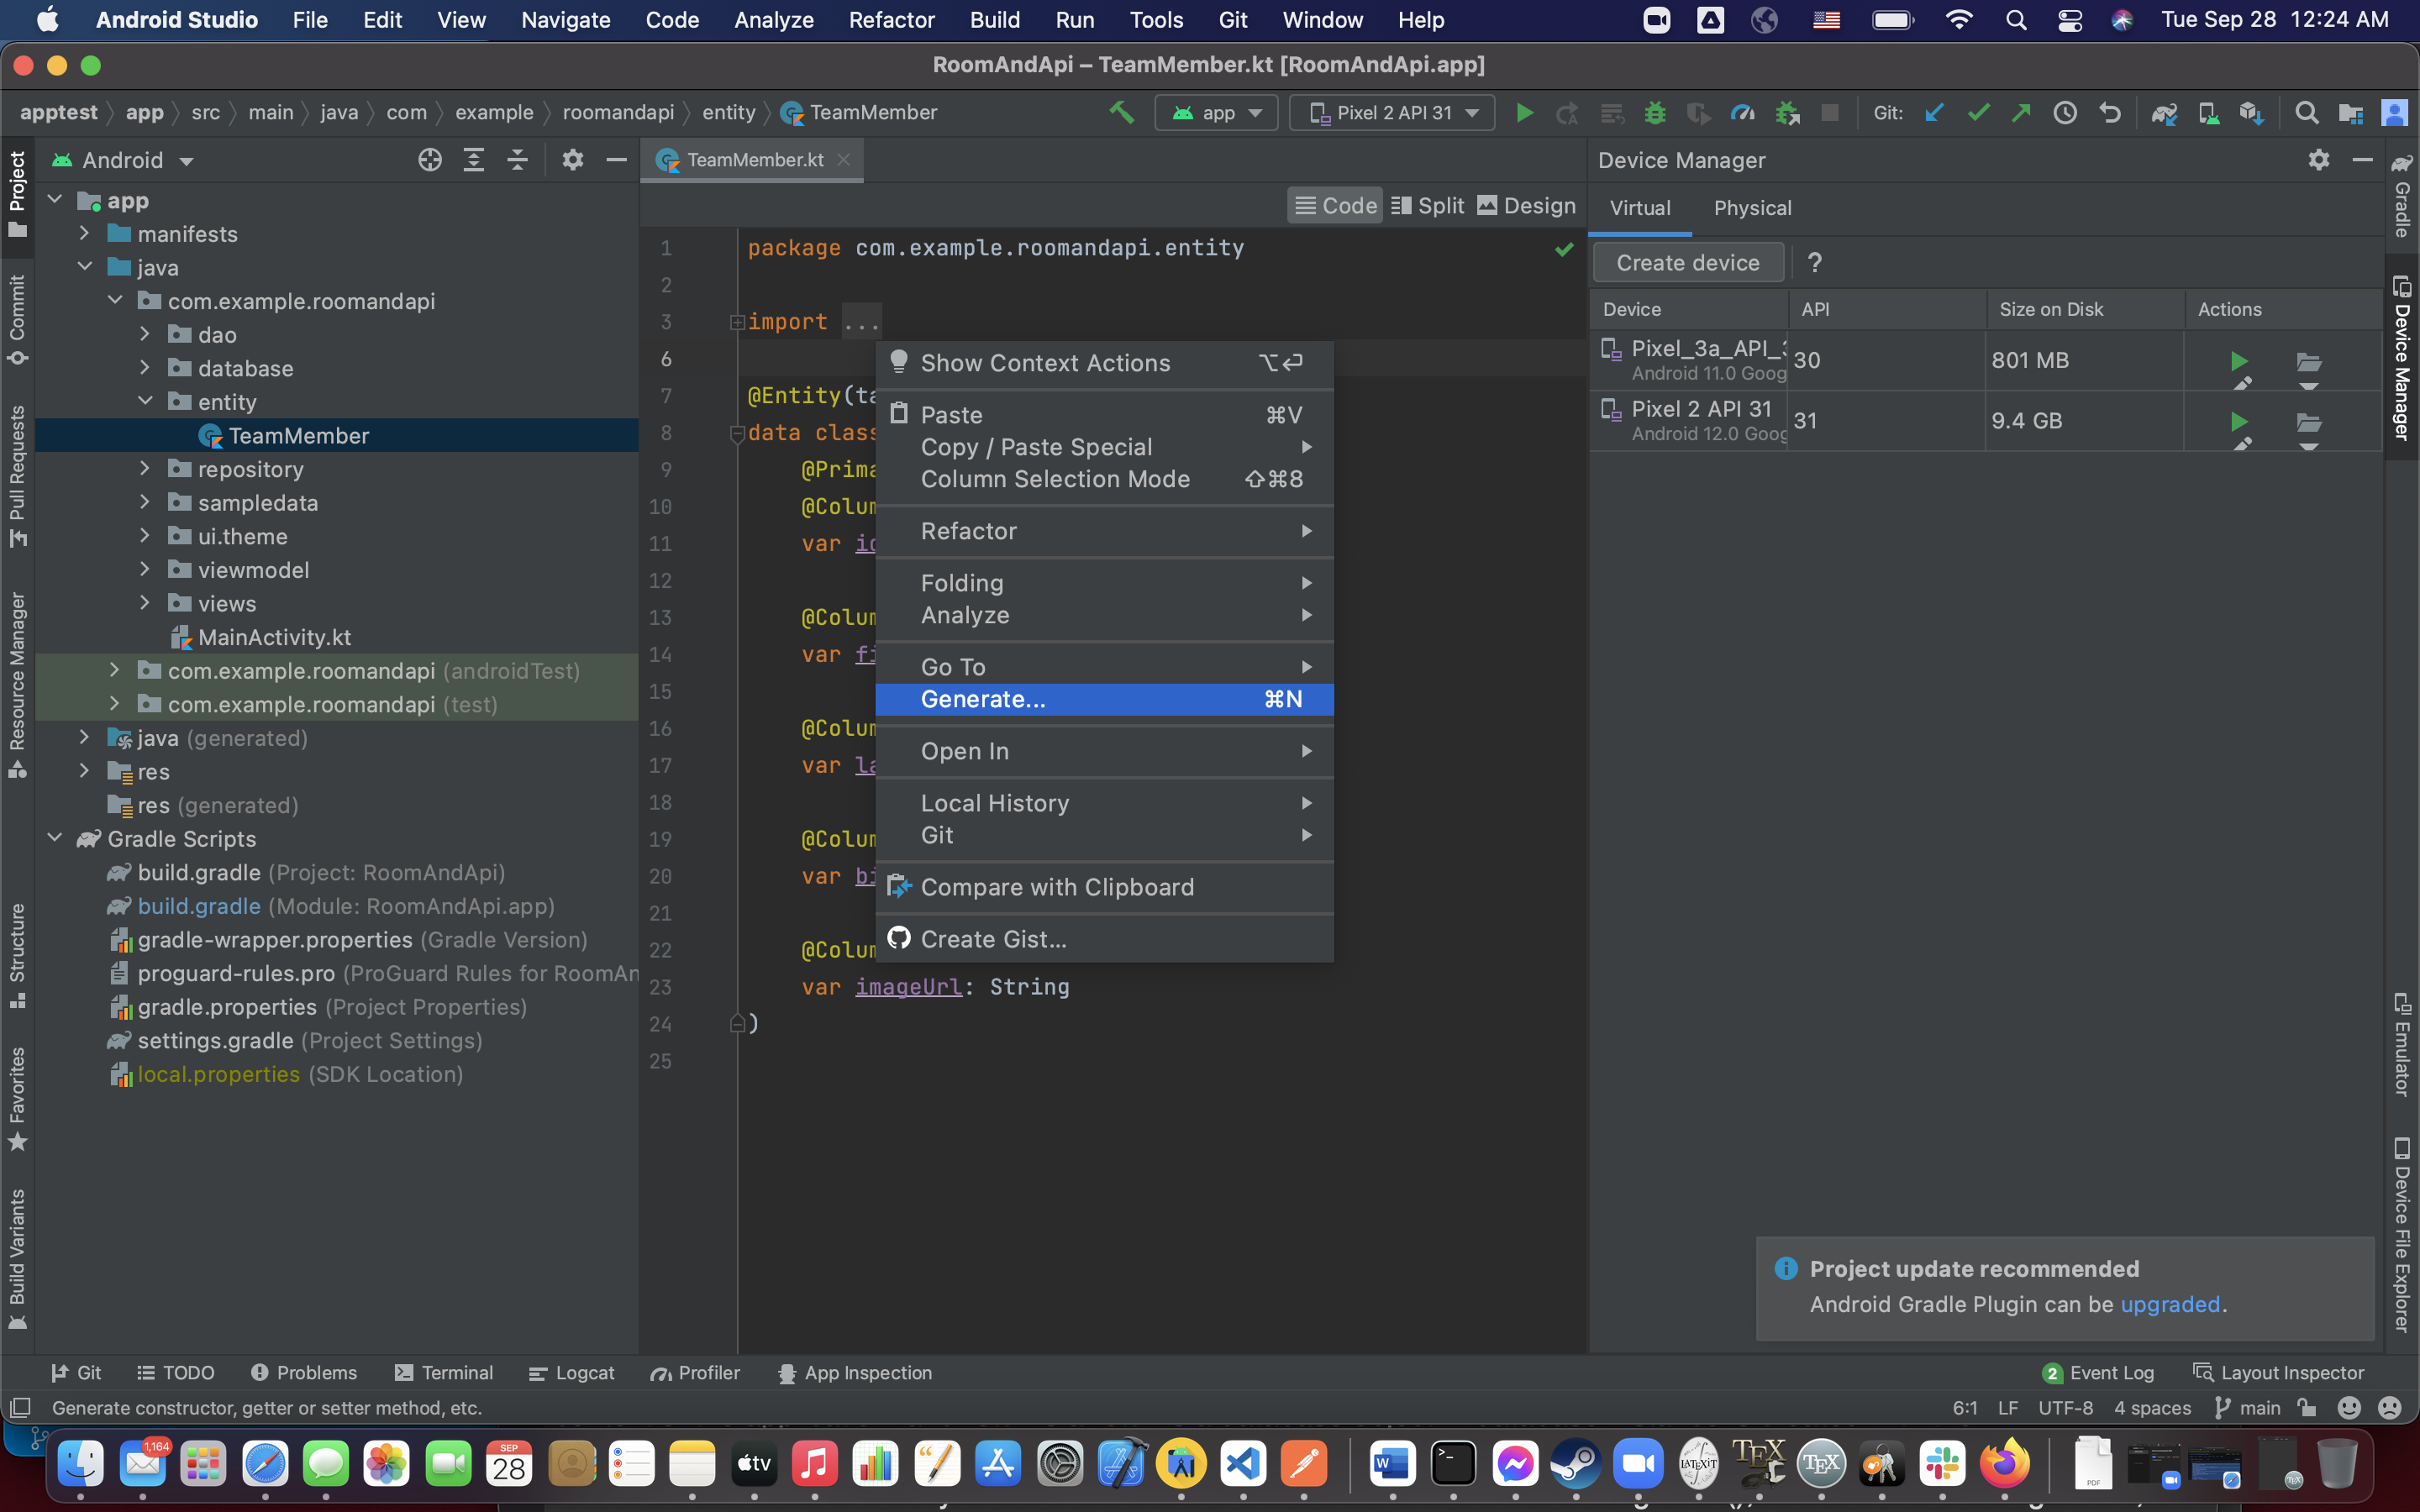
\includegraphics[trim=10 10 10 50, clip, width=\textwidth] {images/testing/1_rightClick.png}
    \caption{Step 1. Open the file you want to test and right click it.}
    \label{fig:test_step_1}
\end{figure}

The process for creating an Android Test with room begins by first navigating to the file that you would like to test. Right click anywhere in the open file and select \verb|Generate...| as shown in Figure \ref{fig:test_step_1}

\begin{figure}[H]
    \centering
    % trim and clip are used to crop the image, trim=left bottom right top
    % width sets max width, height will be scaled appropriately
    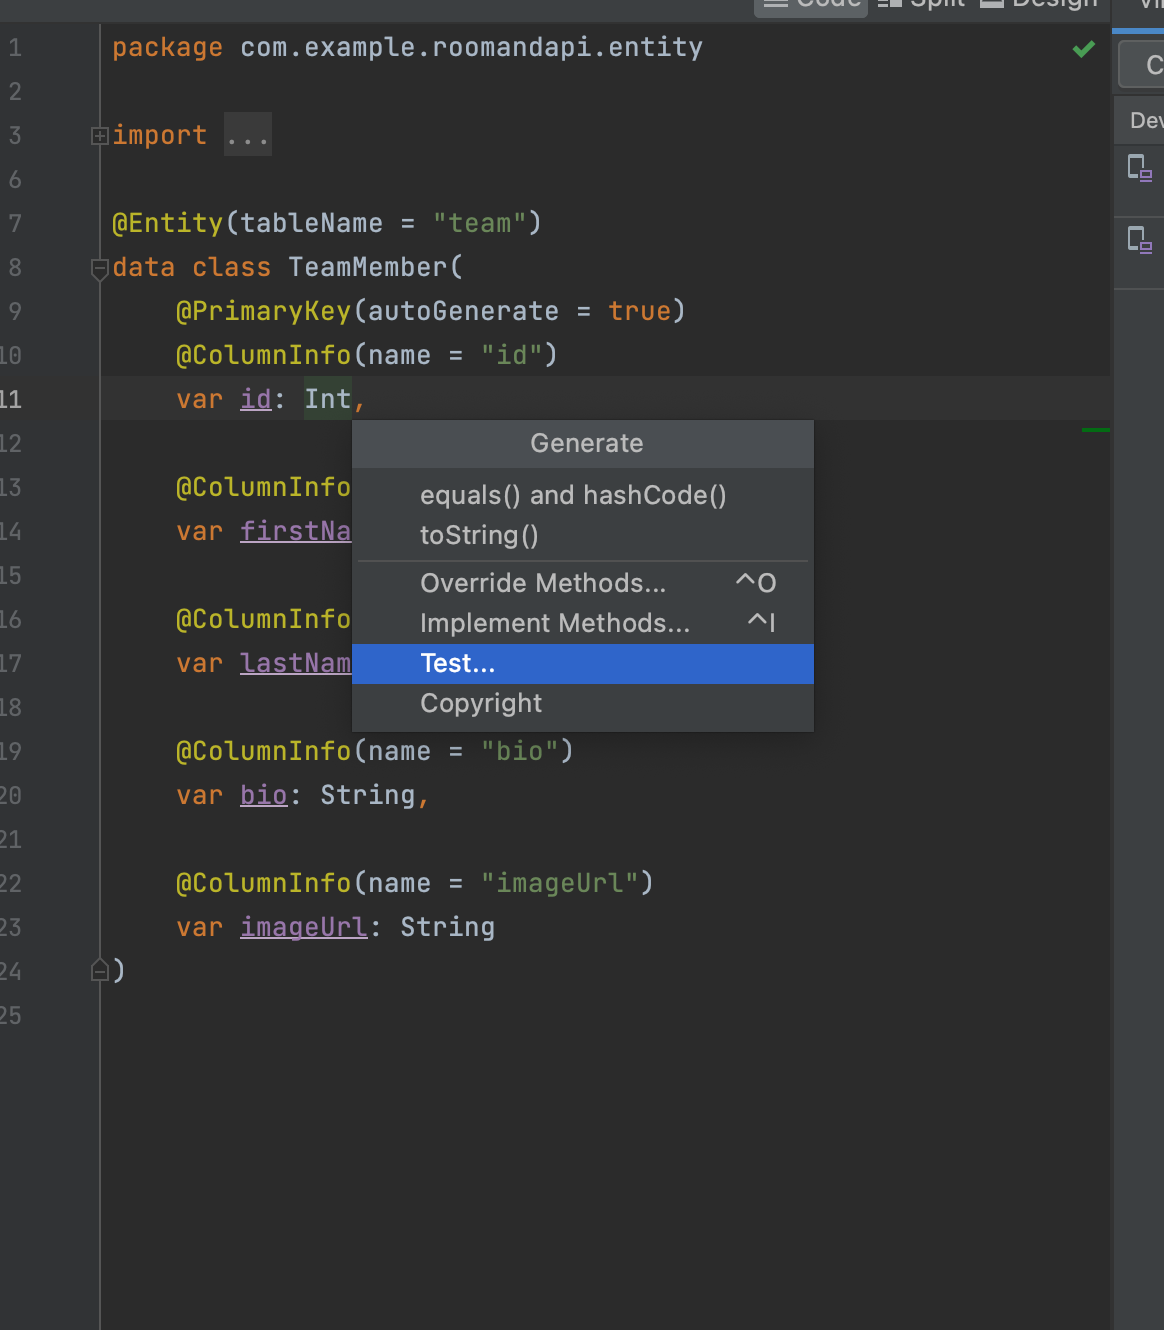
\includegraphics[trim=10 10 10 50, clip, width=\textwidth] {images/testing/2_generate_test.png}
    \caption{Step 2. Click Generate and then Click Test}
    \label{fig:test_step_2}
\end{figure}

From the \verb|Generate| menu, select \verb|Test...| to create a new test file as shown in Figure \ref{fig:test_step_2},

\begin{figure}[H]
    \centering
    % trim and clip are used to crop the image, trim=left bottom right top
    % width sets max width, height will be scaled appropriately
    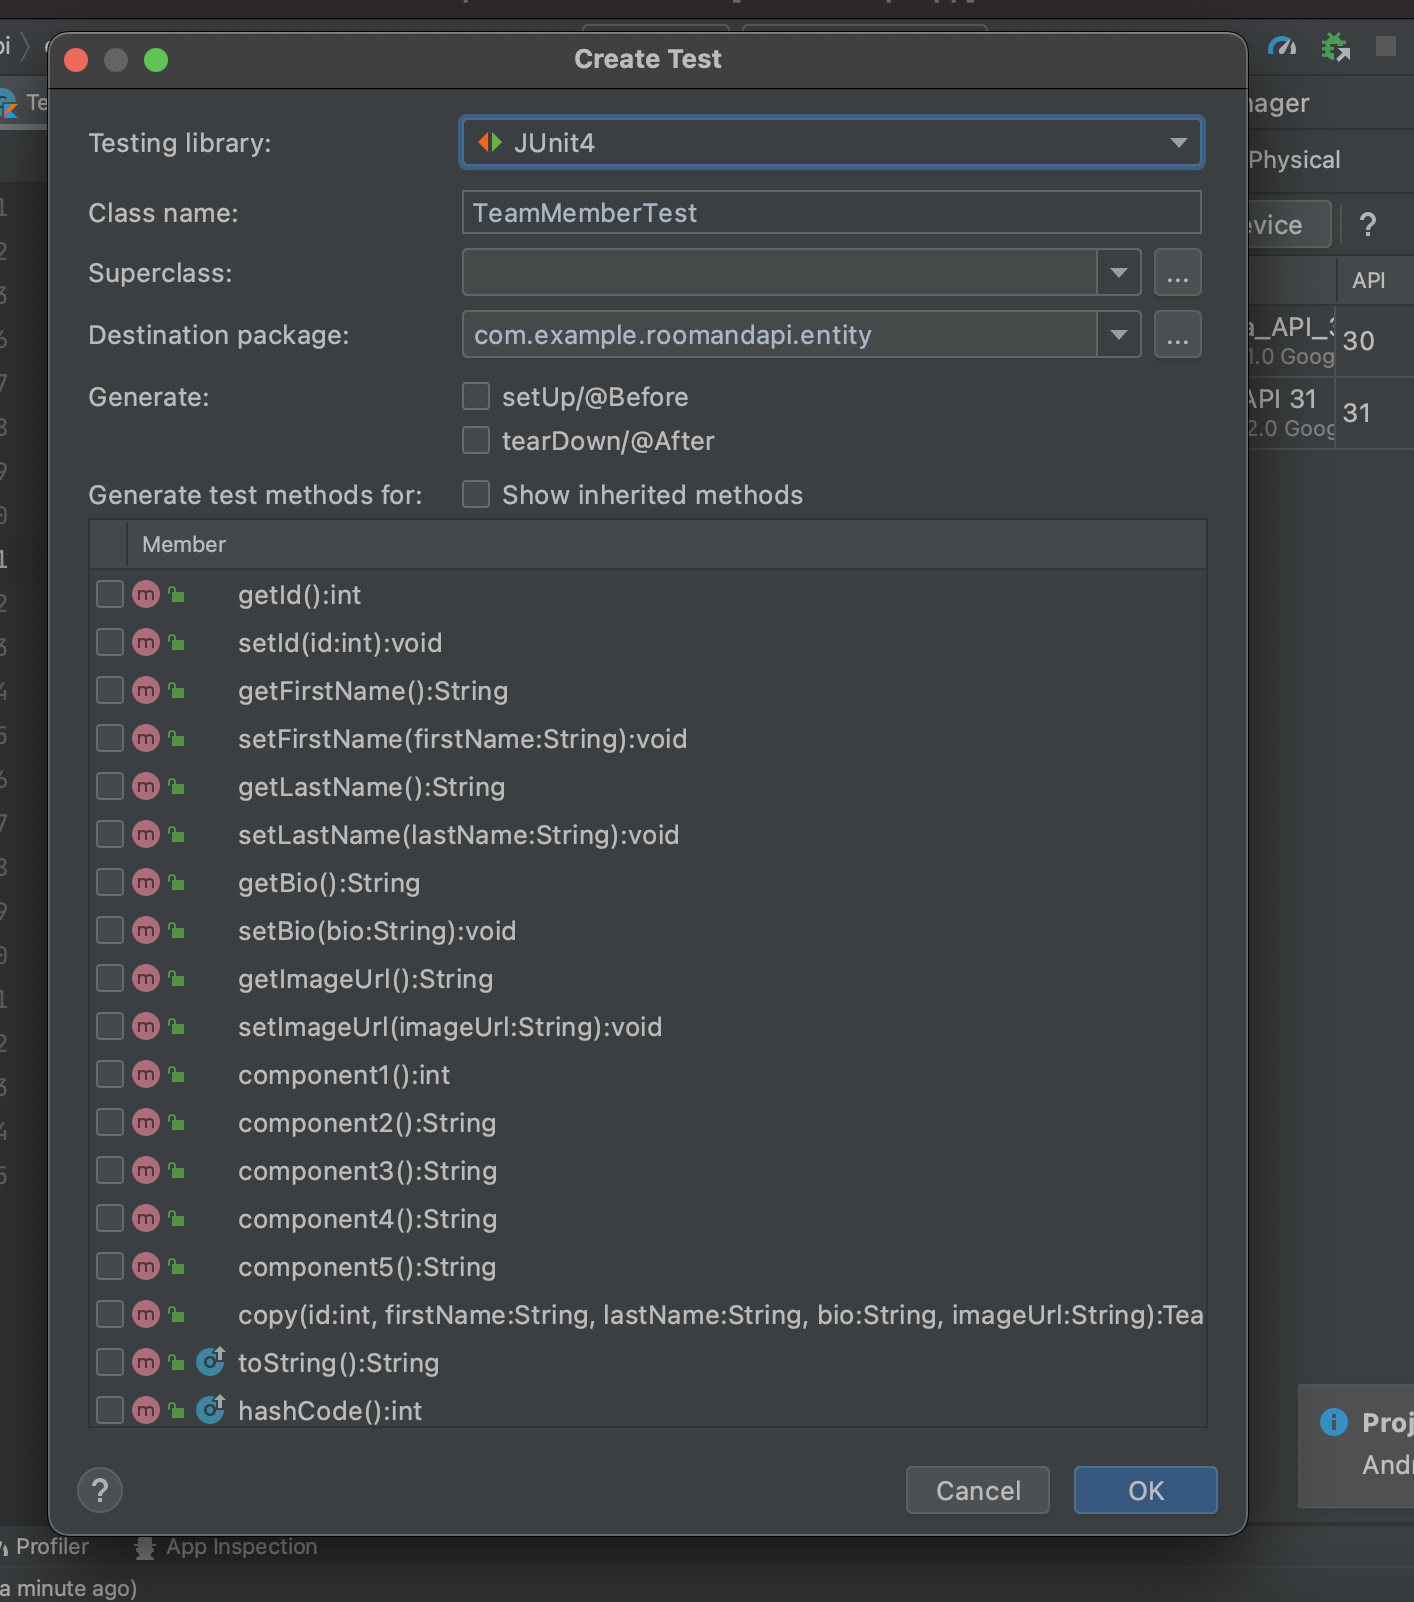
\includegraphics[trim=10 10 10 50, clip, width=\textwidth] {images/testing/3_pick_testing_Framework.png}
    \caption{Step 3, Select the version of JUnit to use}
    \label{fig:test_step_3}
\end{figure}
The \verb|Create Test| dialog box appears after selecting \verb|Test...|. In this dialog as shown in Figure \ref{fig:test_step_3}, the user can specify the type of testing framework to use with the \verb|Testing Library| dropdown. In this example, the JUnit4 testing library is used.

\begin{figure}[H]
    \centering
    % trim and clip are used to crop the image, trim=left bottom right top
    % width sets max width, height will be scaled appropriately
    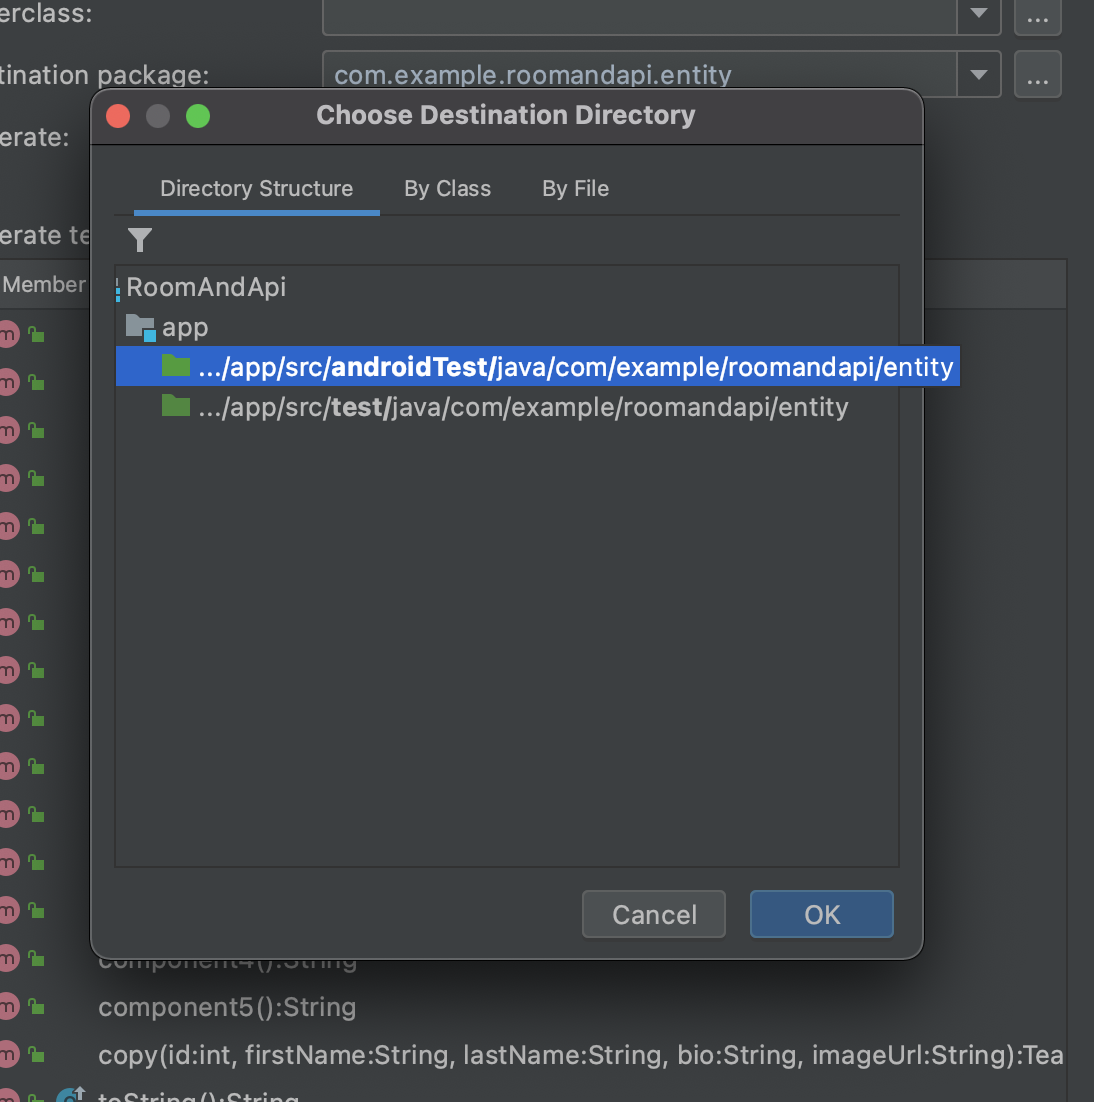
\includegraphics[trim=10 10 10 50, clip, width=\textwidth] {images/testing/4_pick_test_type.png}
    \caption{Step 4, Determine the type of test}
    \label{fig:test_step_4}
\end{figure}
 Then the \verb|OK| button can be clicked to move on to the \verb|Choose Destination| dialog box shown in Figure \ref{fig:test_step_4}. In this dialog box you can specify whether this will be an AndroidTest running within an emulator or a standard JUnit test by selecting the appropriate destination, AndroidTests or Tests. Since we are testing the RoomDatabase, the test has to be an Android Test and must stored in the AndroidTests directory

 \begin{figure}[H]
    \centering
    % trim and clip are used to crop the image, trim=left bottom right top
    % width sets max width, height will be scaled appropriately
    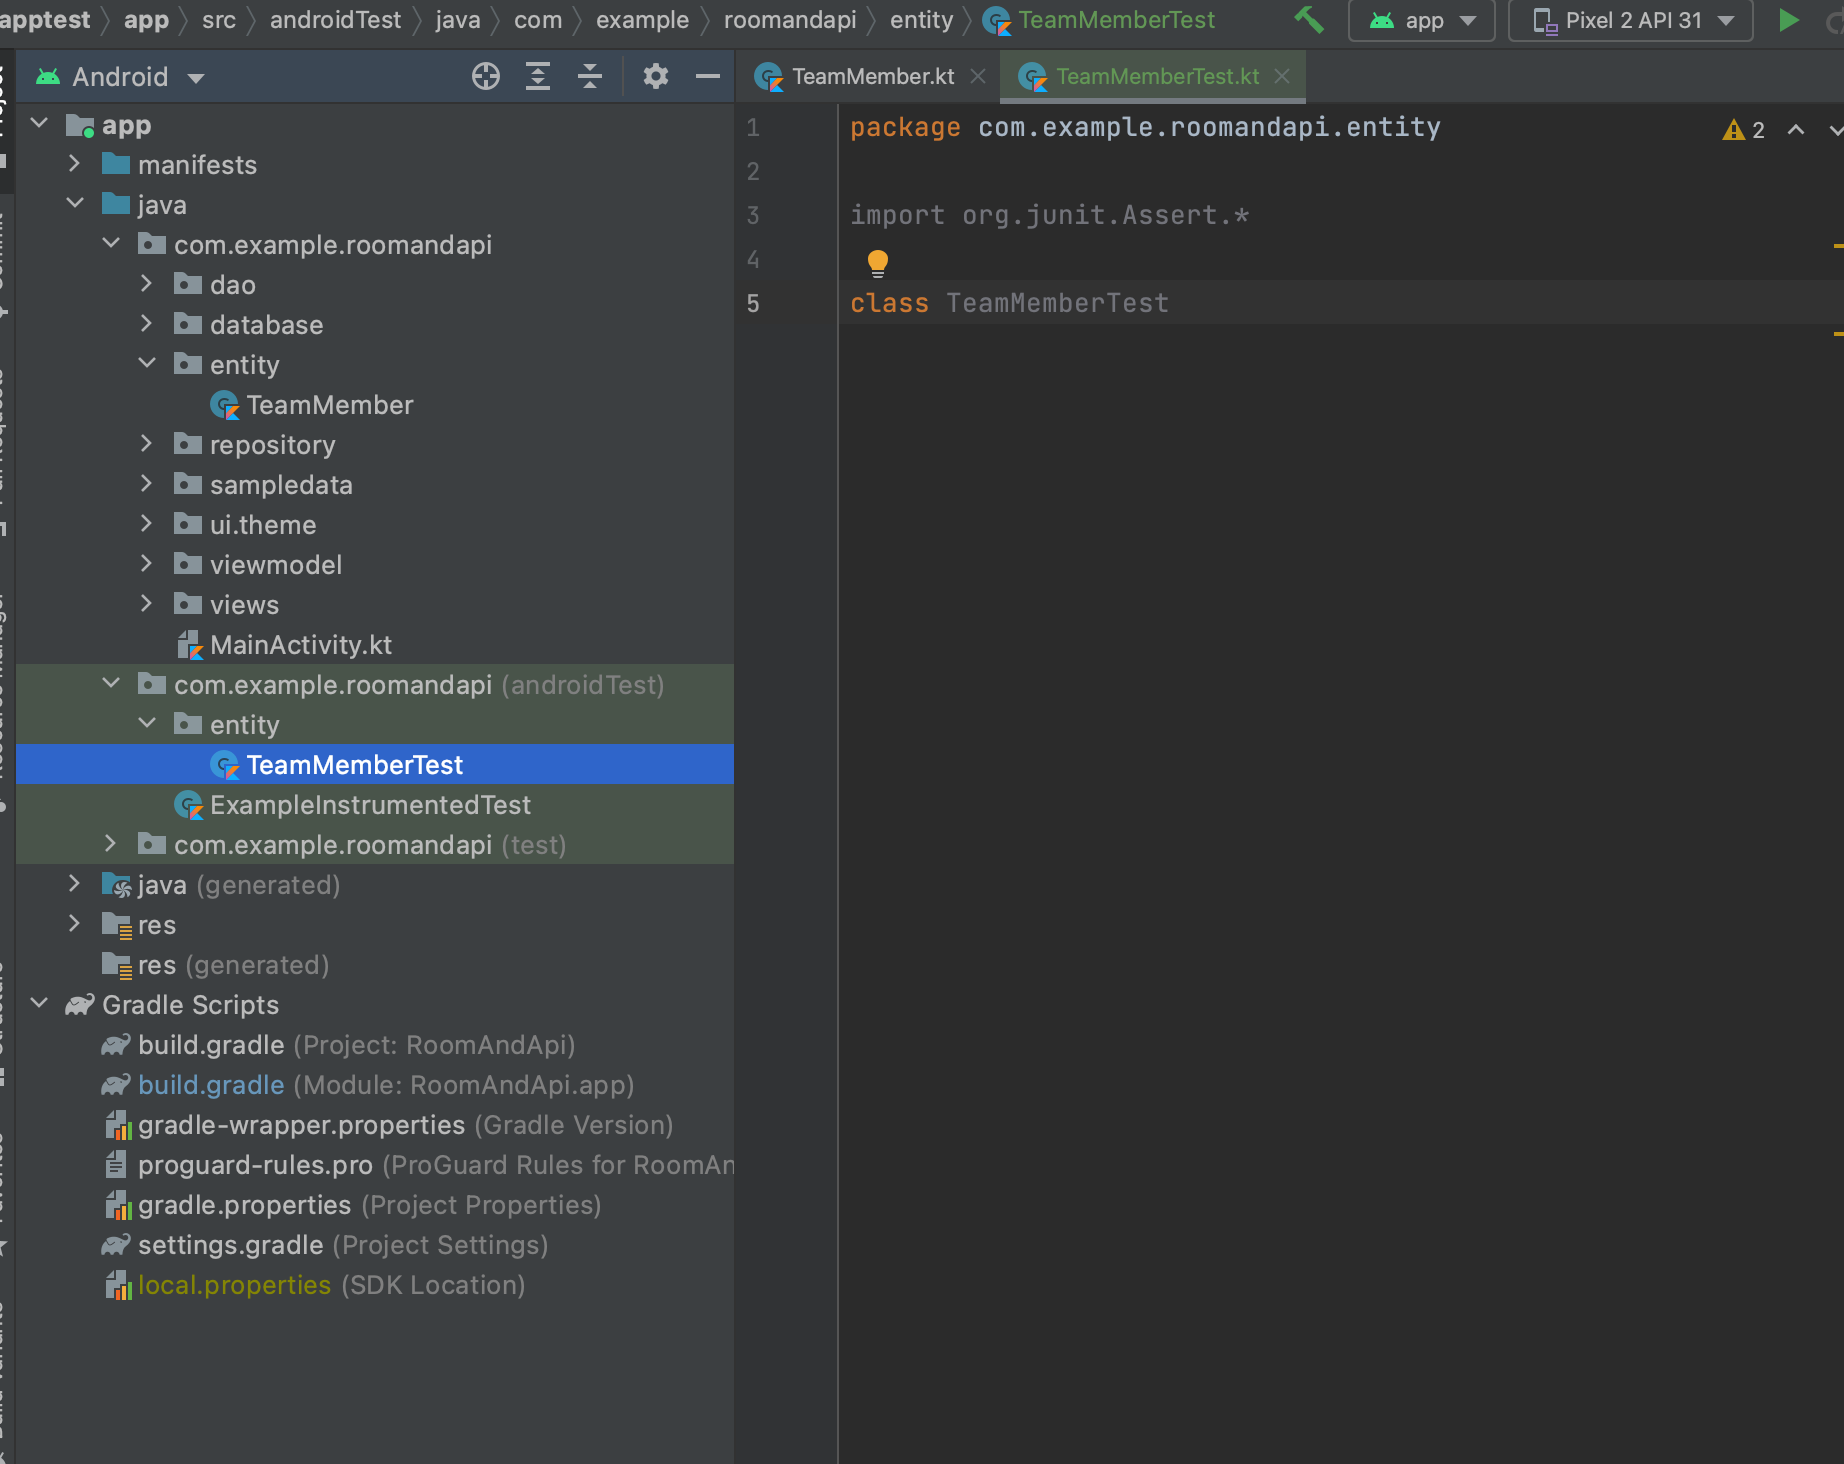
\includegraphics[trim=10 10 10 50, clip, width=\textwidth] {images/testing/5_result.png}
    \caption{Auto-generated Test Class}
    \label{fig:test_step_5}
\end{figure}
 
 After following those steps, a skeleton of an  Android Test class will be created . In order to get the class to run properly, an annotation \verb|@RunWith(AndroidJUnit4::class)| needs to be added at the front of the class. The class header will also need to extend the TestCase class using the heading \verb|class nameOfClass: TestCase(){| After that has been created, common variables need to be created as members of the class. When testing the Room Database, the private members should include an instance of the database, the dao being tested and possibly the repository if the repository is being tested.  

 \begin{lstlisting}[numbers=none, 
			caption=Code to Set up the Database in Test,
			label={lst:before_testing}]
@Before
    public override fun setUp(){
        val context = ApplicationProvider.getApplicationContext<Context>()
        db = Room.inMemoryDatabaseBuilder(context, WCDatabase::class.java).build()
        dao = db.userDao()
    }
\end{lstlisting}
 Since the database will have to be created with every test,  the \verb|@Before| annotation is needed to define the code to generate the database. Listing \ref{lst:before_testing} contains a \verb|setUp()| function which is used to create a an \verb|inMemoryDatabase| which is a database that is loaded into memory but does not persist after it is closed, which makes it ideal for testing. The inMemoryDatabase is created using Room's \verb|inMemoryDatabseBuilder| class which takes the application context and the class of the database to instantiate with the build() method. Once the database is created, the dao is instantiated from the appropriate database method.

   \begin{lstlisting}[numbers=none, 
			caption=Code to close the Database after the test,
			label={lst:after_testing}]
    @After
    fun closeDB(){
        db.close()
    }
\end{lstlisting}

Since every test is going to have to close the databse, the \verb|@After| annotation is used to create a function that is run after each test to close the database. An example of this function is shown in Listing \ref{lst:after_testing}. The function \verb|closeDB()| simply abstracts the database's close method and calls it. 

   \begin{lstlisting}[numbers=none, 
			caption=Example Test for Room Database,
			label={lst:example_room_test}]
    @Test
    fun TestWriteAndReadUser() = runBlocking(){
        val members: List<TeamMember> =  listOf(
            TeamMember(1,
            "Jacob",
            "Conner",
            "Jacob Conner is a senior at Old Dominion University majoring in Computer Science. Currently, he lives in Blacksburg, Virginia, and works in a chat-based technical support role for Dish Network. Some of his hobbies include archaeology, learning Japanese and browsing Linkedin Learning.",
            "https://www.cs.odu.edu/~cpi/old/410/silvers21/bio/Jacob_Conner.jpg")
        )
        dao.insert(members)
        val byName: TeamMember = dao.getByName("Jacob", "Conner")
        MatcherAssert.assertThat(byName, CoreMatchers.equalTo(members[0]))
    }
\end{lstlisting}

Now that the initial setup has been created, tests for the database can be created. A test is annotated with  \verb|@Test| before the test function.  Each function is set up with runBlocking to force the thread used to call the test to wait until the test finishes \cite{kotlinCoroutines}.  Then the test is setup with anything particular to the test. In Listing \ref{lst:example_room_test} the database's ability to insert and read data is tested by creating an instance of a team member. This team member is inserted into the database using the dao's insert method. The database is read to create a new instance of the team member which should be the same as the team member just inserted with the dao's getByName method. The MatcherAssert.assertThat method is used to test if the two TeamMember entities are equal. If they are equal, the test passes \cite{SimplifiedCodingRoomTesting}. 

\lstinputlisting[language=Java, caption=Example entity test class, label={lst:exampleEntityTest}]{app/src/androidTest/java/com/example/roomandapi/entity/TeamMemberTest.kt}

The example test file for the TeamMember class is shown in listing \ref{lst:exampleEntityTest}. 


\section{JetPack Compose}

\subsection{Navigation}
Navigation in JetPack Compose consists of a NavController to provide the routes to the various views and buttons on the view to navigate to those routes \cite{mediumJetpackNavigation} \cite{NavigationCodeLab}. 
\lstinputlisting[language=Java, caption=Example Activity View with a NavController, label={lst:exampleNavView}]{app/src/main/java/com/example/roomandapi/views/MainView.kt}


\begin{lstlisting}[numbers=none, 
			caption=Function to create a simple Nav Controller,
			label={lst:navControllerFunction}]
@Composable
fun appNavController() {

    val navController = rememberNavController()
    //default destination
    NavHost(navController, startDestination = "nameOfDefaultRoute") {
    	//list routes
        composable(route = "<nameOfFirstRoute>") {
        	    //viewToLoad
	    firstView(navController)
        }
        
        composable(route = "<nameOfSecondRoute>") {
	    secondView(navController)
        }
    }
}
\end{lstlisting}

In the navController function shown in listing \ref{lst:navControllerFunction}, the navController begins like all composable functions with the \verb|@Composable| annotation. Then the name of the function for the navController is defined. Since the nav controller manages routes, a state variable needs to be handled to keep track of the current route. This state is defined as navController in the example code and is created using the \verb|rememberNavController()| method. Next the NavHost is created which takes the state, and the default or \verb|startDestination|. Within the NavHost function, the \verb|composable| method is called for each route. This method simply takes the route which has a string for the name of the route. Inside of this function, the view that should be loaded with that particular route. Since we need to keep track of the current route, each view used in a navController should require the remembered navController..  
\begin{lstlisting}[numbers=none, 
			caption=Button to navigate to a view,
			label={lst:navButton}]
Button(onClick = { navController.navigate("<routeToNavigateTo") }) {
                //Label for button
                Text("Name of Button")
            }
}
\end{lstlisting}

In order to move between routes, a Button component can be created like the one shown in Listing \ref{lst:navButton}. To make the button switch to a different route, the \verb|onClick| argument needs to be set to \verb|navController.navigate("nameOfRoute")|. Then normal styling can be used inside of the button. For example, a label can be set with the Text component with the Text property set to the name of the button. The text property's \verb|text=| can be omitted when the text is the only property set \cite{mediumJetpackNavigation}.  

\subsection{Handling Remote Resources - Images}
\begin{lstlisting}[numbers=none, 
			caption=Coil Dependency,
			label={lst:coilDependency}]
implementation("io.coil-kt:coil-compose:1.3.1")
\end{lstlisting}
Some APIs may make use of Image files referred to remotely and there are instances when we would like the application to download an image from the web and use that image in the web. In order to support this, the \verb|Coil| library can be imported by adding the dependency in Listing \ref{lst:coilDependency} into the application's \textit{build.gradle} file. 

\begin{lstlisting}[numbers=none, 
			caption=Example Image using Coil,
			label={lst:exampleWithCoil}]
Image(
                        painter = rememberImagePainter("https://www.cs.odu.edu/~cpi/old/410/silvers21/bio/Jacob\_Conner.jpg"),
                        contentDescription = null,
                        modifier = Modifier.size(128.dp)
                    )
\end{lstlisting}


Once the dependency has been imported, the image urls can be loaded in the app by creating an \verb|Image| composable function and setting the painter property with the \verb|rememberImagePainter| function that takes the url as an argument \cite{StackOverflowCoil}. An example image composable to load a remote resource is shown in Listing \ref{lst:exampleWithCoil}.

\subsection{Creating a form}

A common task in most mobile applications is retrieving input from the user and this is most commonly handled through forms. Forms are a collection of various input fields and at least one button, which is used to trigger the submission process where the inputs are retrieved from the form, processed and then sent to a database or the relevant processing tools. 
\lstinputlisting[language=Java, caption=Example View with a form to collect projects that a team member may work on, label={lst:exampleForm}]{app/src/main/java/com/example/roomandapi/views/AddProjectVIew.kt}

An example of a form created using JetPack Compose is shown in Listing \ref{lst:exampleForm}. This form is a bit contrived to providet a variety of the more common input, but it is used to collect information about projects that a team member may work on. The form first consists of a text field to get the name of the project, a set of radio buttons that a user can use to select the perceived difficulty of the project, a dropdown box to set the category of project, a date for when the. project was created and lastly a drop down box where the user can specify the team member assigned to it, and it will return the user id in the team table for that team member. 


The code used to create the form is shown in the AddProjectView function. This function is a composable function that is used in other composable functions and makes use of other other composable functions, so the \verb|@Composable| annotation is used. so it makes use of the @Composable which is accessible by a route in the NavController, so the NavController has to be passed to the function. 
\begin{lstlisting}[numbers=none, 
			caption=Creating a ViewModel in a View,
			label={lst:creatingAViewModelInView}]
    val context = LocalContext.current
    val projectViewModel: ProjectViewModel = viewModel(
        factory = ProjectViewModelFactory(context.applicationContext as Application)
    )
\end{lstlisting}

Since the form will have to insert the user's input into a database, the ProjectViewModel is created using the code shown in \ref{lst:creatingAViewModelInView}. ViewModels require the context of the application, so the context variable is created using the LocalContext.current to get the context of the current view. A \verb|ProjectViewModel| defined in the \verb|viewmodel/ProjectViewModel.kt| class is created using the ProjectViewModelFactory method with the context variable. The resulting projectViewModel value can now be used in other parts of the view to make use of the various CRUD operations in that view model. 

\begin{lstlisting}[numbers=none, 
			caption=Tracking State Changes,
			label={lst:trackState}]
 //remember the values in the form
    var projectName by remember { mutableStateOf("") }
    val projectTypeState = remember { mutableStateOf("")}
    val difficulty = remember { mutableStateOf("") }
    val dateValue = remember { mutableStateOf("") }
    val UserID = remember { mutableStateOf(0)}
    val UserIDString = remember { mutableStateOf("")}
\end{lstlisting}
Since JetPack Compose makes use of states to track changes in values of the various fields in our form, a number of mutable states need to be created using the \verb|remember{ mutableStateOf("") }| function. These can then be passed to the values of textFields, dropDowns and radio buttons and are frequently manipulated using the \verb|onValueChange| property of those fields using code like \verb|onValueChange = { myState.value = it }|, which can be used to tell the field to automatically update the value property of the state when the user enters input in that particular field. There should be at least one state per input field in the form and certain inputs may make use of more if the input field has to trigger a dialog box or a dropdown menu. The states used to track the values in the AddProjectForm are shown in Listing \ref{lst:trackState}

\subsubsection{Rows and Columns}
Now that the initial discussion on state and using viewmodels in a view has been provided, the process of creating the form and the elements in it will be discussed. In JetPack Compose there are a variety of containers to organize elements on a screen, but the two most common are \verb|Column()| and \verb|Row()|. Columns arrange elements vertically and rows arrange elements horizontally. Both Column and Row take a variety of optional arguments that can be used to further customize the layout of the composable function. In this example form, I have stored all of the elements in a Column that fills up the width of the screen using the \verb|Modifier.fillMaxWidth()| property with the exception of a left and right margin set to 30.dp using the \verb|Modifier.padding(start=30.dp, end=30.dp)| property. 
At the top of the form, which is the first element in the Column composable, the navigation elements are stored in a Row() where buttons to go to the main screen, about us screen and the add a project screen. These buttons are placed immediately after each other, so they are placed touching each other from right to left. 

\subsubsection{Spacers}

\begin{lstlisting}[numbers=none, 
			caption=Using Spacers,
			label={lst:spacer}]
 Spacer(modifier = Modifier.padding(top = 30.dp))
\end{lstlisting}
In order to create white space between various elements a spacer can be used. A spacer takes a modifier argument which can be set to the Modifier object with a property. In Listing \ref{lst:spacer} the spacer has a top margin of 30.dp which is used to provide 30.dp units of white space between the navigation and the next element. 
\sububsection{Text}
A title can be created for the form using a \verb|Text()| element. There are several properties that can be set for the text property which can used to style the text, but at a minimum it requires an argument of text which is the string displayed for the text. 
\subsubsection{Centering}
\begin{lstlisting}[numbers=none, 
			caption=Centered Text,
			label={lst:centeredTitle}]
  //Create a heading
        Row(
            Modifier
                .fillMaxWidth(),
            horizontalArrangement = Arrangement.Center

        ) {
            Text(text = "Add a Project")
        }

\end{lstlisting}
If we simply place the text element in the column, we will find the text element is left aligned with a padding of 30.dp. Generally, a centered title is more visually appealing, so we can create a Row container and make use of the Modifier.fillMaxWidth() property and the horizontalArrangement = Arrangement.Center property to create a row where all items in that row are center aligned. Then the text for our title can be stored inside this Row container as shown in Listing \ref{lst:centeredTitle}. 

\subsubsection{TextField Inputs}

\begin{lstlisting}[numbers=none, 
			caption=TextField inputs,
			label={lst:textField}]
  TextField(value = projectName,
                onValueChange = { projectName = it }
            )
\end{lstlisting}

Now that a title has been created, we can start creating the various input types needed for our form. The first input in this form is the text input field used to get the name of the project. Generally forms make use of a label before the input field, so I opted to create a Row container for each input that consisted of a \verb|Text| field with the name of the field, a spacer with a padding of 10.dp and then the input type of interest. Since project name is a text field, the TextField composable is used as shown in Listing \ref{lst:textField}. TextFields have at least two arguments, a value argument which points to the state used to track this field and the onValueChange which is used to update the value of that state. 

\subsubsection{RadioButtons} 

\begin{lstlisting}[numbers=none, 
			caption=Radiobutton inputs,
			label={lst:radioButton}]
@Composable
fun GroupedRadioButton(mItems: List<String>, radioState: MutableState<String>) {

    Row(Modifier
        .fillMaxWidth()) {
        mItems.forEach { mItem ->
                RadioButton(
                    selected = radioState.value == mItem,
                    onClick = { radioState.value = mItem },
                    enabled = true,
                    colors = RadioButtonDefaults.colors(selectedColor = Color.Magenta)
                )
            Text(text = mItem, modifier = Modifier.padding(start = 8.dp))
        }
    }
}
            )
\end{lstlisting}
The second input type used in the form is the radio button which is used to specify the perceived difficulty of the project. Since there were more than a few lines of code to create a radio button, a GroupedRadioButton function was created to store a list of strings for the various options to display and the mutableState used to track the value of the radiobutton after any changes. The GroupedRadioButton composable function is shown in Listing \ref{lst:radioButton}

\begin{lstlisting}[numbers=none, 
			caption=DropDown box,
			label={lst:projectDropDown}]
@Composable
fun ProjectTypeDropdown(projectTypeState: MutableState<String>) {
    var expanded by remember { mutableStateOf(false) }
    val items = listOf("Personal Project", "School Project", "Work Project")
    var selectedIndex by remember { mutableStateOf(0) }
    Box(modifier = Modifier.wrapContentSize(Alignment.TopStart)) {
        Text(items[selectedIndex],modifier = Modifier
            .fillMaxWidth()
            .clickable(onClick = { expanded = true })
            .background(
                Color.LightGray
            )
        )
        DropdownMenu(
            expanded = expanded,
            onDismissRequest = { expanded = false },
            modifier = Modifier
                .fillMaxWidth()
                .background(
                    Color.LightGray
                )
        ) {
            items.forEachIndexed { index, s ->
                DropdownMenuItem(onClick = {
                    selectedIndex = index
                    expanded = false
                    projectTypeState.value = items[selectedIndex]
                }) {
                    Text(text = s)
                }
            }
        }
    }
}
\end{lstlisting}


\subsubsection{Dropdown Boxes}
A dropdown or select box can be used to select one option from a list of options, much like radio buttons. The advantage to dropdown boxes is that they make better use of space and can store more options on a screen through the ability to scroll down a list of different options, whereas  all radio buttons have to be displayed at once which limits their use to cases where only a few options are available. In this form there are two dropdown boxes, one is used to select the type of project, personal, school or work and the other is to select the name of a user and it returns the id fo the user. The biggest difference in the implementation of these two drop downs is that the UserDropDown box creates a TeamMemberViewModel and uses it to populate a list of TeamMember objects to get the names and ids of all team members. Since a query to the database is used and there could be some delay, conditional logic has to be used for the currently selected value to be an empty string if  the list is empty. Otherwise the application will crash due to an invalid index in the list. In Listing \ref{lst:projectDropDown}, the code to create the project dropdown box is shown. In this function, three mutable states are used. First the expanded mutable state tracks a boolean to see if the dropdown is open or not and is set to true when clicked. The second mutable state, selectedIndex, is used to track an integer equal to the index of the currently selected list item in the dropdown box. The last mutable state is projectTypeState which is the state passed to the function and is used to track the current string value of the item at the selectedIndex. A box container containing a single text element is used to define the appearance of the dropdown field when it is closed. The \verb|DropdownMenu| container is used to define the appearance of the dropdown menu when it is clicked and the list of all dropdown items is shown. Inside of this function, the list items are looped and \verb|DropdownMenuItem|s are created from that list each with an \verb|onClick| method which is used to set the values of the various states needed in the Dropdown function. A text element inside of the DropdownMenuItem is used to set the text displayed for that item in the dropdown menu. 

\subsubsection{DatePicker}
The last type of input field in the AddProjectView is the DatePicker input. JetPack Compose does not natively support a DatePicker, but it can be implemented using a third party library such as Compose Material Dialogs \cite{GitHubComposeMaterialDialogs}.  

\begin{lstlisting}[numbers=none, 
			caption=Compose Material Dialogs Dependencies,
			label={lst:composeMaterialDialogDependencies}]
  implementation "io.github.vanpra.compose-material-dialogs:datetime:0.6.0"
  implementation "io.github.vanpra.compose-material-dialogs:color:0.6.0"

\end{lstlisting}
To use this library the dependencies shown in Listing \ref{lst:composeMaterialDialogDependencies} need to be added to the \verb|app/build.gradle| file. 

\begin{lstlisting}[numbers=none, 
			caption=DatePicker ,
			label={lst:datePicker}]
  @Composable
fun showDatePicker(DateValue: MutableState<String>){

    val dialogState = rememberMaterialDialogState()
    val textState = remember { mutableStateOf(TextFieldValue()) }
    val dialog = MaterialDialog(
        dialogState = dialogState,
        buttons = {
            positiveButton("Ok")
            negativeButton("Cancel")
        }){
        datepicker { date ->
            val formatter = DateTimeFormatter.ISO_LOCAL_DATE
            val formattedDate = date.format(formatter)
            textState.value = TextFieldValue(formattedDate)
            DateValue.value = formattedDate
        }
    }
        Column(modifier = Modifier.padding(16.dp)) {
        ReadonlyTextField(
            value = textState.value,
            onValueChange = { textState.value = it },
            onClick = {
                dialogState.show()
            },

            label = {
                Text(text = "Date")
            }
        )
    }
\end{lstlisting}

The DatePicker function is created using the code shown in Listing \ref{lst:datePicker}. \cite{GrobmannDatePicker}. This code basically creates a dialog box using the MaterialDialog function and then a datepicker function is used to take the date selected and convert it to a string. After the dialog box has been created, the dialog state's  \verb|show| method needs to be called with an onclick event to be able to show the dialog box. 
\begin{lstlisting}[numbers=none, 
			caption=ReadonlyTextField ,
			label={lst:readonlytextfield}]
@Composable
fun ReadonlyTextField(
    value: TextFieldValue,
    onValueChange: (TextFieldValue) -> Unit,
    modifier: Modifier = Modifier,
    onClick: () -> Unit,
    label: @Composable () -> Unit
) {
    Box {
        TextField(
            value = value,
            onValueChange = onValueChange,
            modifier = modifier,
            label = label
        )
        Box(
            modifier = Modifier
                .matchParentSize()
                .alpha(0f)
                .clickable(onClick = onClick),
        )
    }
}
\end{lstlisting}
 In this case a custom textField class, called \verb|ReadonlyTextField| shown in Listing \ref{lst:readonlytextfield} is used to create a clickable text element that can show the resulting date text, but does not trigger the keyboard. In this class a box element with a text field and a box element over top of the text field is used to prevent triggering the keyboard, so it has the ability to behave like a button, but also dynamically updates the text value when the datePicker is closed \cite{GrobmannDatePicker}. 

\subsubsection{Submit Button}
\begin{lstlisting}[numbers=none, 
			caption=Submit Button ,
			label={lst:submitButton}]
 Row(horizontalArrangement = Arrangement.Center,
        modifier = Modifier.padding(start = 120.dp, end = 120.dp)) {
            Button(onClick = { submit(projectName, difficulty.value,
                                     projectTypeState.value, dateValue.value,
                                     UserID.value, projectViewModel) }){
                Text("Submit")
            }
        }
\end{lstlisting}
The last element of the AddProjectView is the submit button. This is created using a \verb|Button| with an onClick argument set to the function used to submit the form data. The label for the button is set by storing a \verb|Text| element inside of the button. The code used to create the submit button is shown in \ref{st:submitButton}
\subsubsection{Submit Button}
\begin{lstlisting}[numbers=none, 
			caption=Submit Function ,
			label={lst:submitFunction}]
 fun submit(projectName: String, difficulty: String,
           projectType:String, dateValue:String, UserID: Int, projectViewModel: ProjectViewModel ){

    val formatter = DateTimeFormatter.ISO_LOCAL_DATE
    val date: LocalDate = LocalDate.parse(dateValue, formatter)
    var project = ProjectEntity(1, projectName, difficulty, projectType, date, UserID)
    projectViewModel.addProject(project)
}
\end{lstlisting}
The submit function simply takes the value for each of the mutableStates that was tracking an input field and then viewModel used to insert the data into the database. The various values are used to create a ProjectEntity and then the ProjectViewModel's addProject method is used to add the entity to the database. The code used to create the submit function is shown in Listing \ref{lst:submitFunction}

\section{Documenting with Dokka}
test
\begin{appendix}
  \listoffigures
  \newpage
  \listoftables
  \newpage
  \lstlistoflistings

\end{appendix}
\newpage
\RaggedRight
\bibliography{references}{}
 \bibliographystyle{elsarticle-num} 
\end{document} 